% Chapter 1

\chapter{Introduction} % Main chapter title

\label{Chapter1} % For referencing the chapter elsewhere, use \ref{Chapter1} 

%----------------------------------------------------------------------------------------

% Define some commands to keep the formatting separated from the content 
\newcommand{\keyword}[1]{\textbf{#1}}
\newcommand{\tabhead}[1]{\textbf{#1}}
\newcommand{\code}[1]{\texttt{#1}}
\newcommand{\file}[1]{\texttt{\bfseries#1}}
\newcommand{\option}[1]{\texttt{\itshape#1}}

%----------------------------------------------------------------------------------------

\section{Background}
\subsection{Computing In Research}
Computing as a means to understand data has been around for a long time. As with all other technology, advancements in computing have resulted in more affordable systems which directly benefit computational research fields. Some of these advancements will be discussed in the subsequent sections.

%----------------------------------------------------------------------------------------

\subsection{Problem Statement}

Modern technology is enabling the generation of more data in areas where it was not possible before. Pricing for specialised tools such as automated genome sequencers is lowering every year and enabling the data generation in smaller research groups to grow significantly \parencite{jagadish2014big}. Many laboratories across different regions are also generating data that may be of value to other researchers, which may need to be shared \parencite{marx2013biology}. With the increase in scale and size of data sets, structured or unstructured, it is becoming increasingly difficult for researchers to move the data to facilities that allow for processing due to factors such as time and cost of data transfer \parencite{marx2013biology}.

Cloud computing has aided in preventing institutions from having to pour exorbitant amounts of money into the purchase and maintenance of computing infrastructure. This has allowed many small to large industrial and research firms to process more data at less expense. The issue of moving data remains. Once data to be processed reaches the order of terabytes (approx. 10\textsuperscript{12} bytes) or petabytes (approx. 10\textsuperscript{15} bytes) and in-turn yield data which is large, it becomes unrealistic to upload to and download from external sites.

With cloud computing becoming more prevalent, the concept of data regulation and privacy plays a bigger role. Biological data, especially that of humans, has strict regulations regarding whom are allowed to access the data and where the data is geographically allowed to be used. This potentially introduces hurdles when trying to use cloud computing services as there is no guarantee that a provider has data centers that are located in the correct geographic areas.

If cloud computing environments can be used, system administrators need to manage the various virtual machine deployments and software packages for each of the researchers they cater to, unless the researchers are tasked to use the cloud environment directly themselves. The use of a cloud environment in this manner can be an increasingly complex and time consuming task.

%----------------------------------------------------------------------------------------

\subsection{Data}

Data storage devices have become considerably cheaper \parencite{backblaze}. This has allowed many institutions to keep up with the growing amount of research data that gets generated by modern sensor devices.

However, the trend for larger-scale data generation is causing an increasing issue of sharing across institutions. The sharing of data is a staple of the scientific community. It allows researchers to make new observations on a data set used for another purpose, or allows the verification of results \parencite{birnholtz2003data}. Modern national and international networks are falling behind in terms of speed, resulting in substantial waiting periods for researchers to share data. With an increasing number of modern research projects being collaborative, researchers are proposing new ways of sharing and co-locating data \citep{foster2003virtual,zhao2006virtual,pavlo2009comparison,winter2007electronic}.

%----------------------------------------------------------------------------------------

\subsection{Virtualisation}
In today's world, virtualisation is an integral technique that is implemented by many organisations of various sizes in order help maintain different services and applications. Two major types of virtualisation are traditional virtual machines (hypervisor-based) and containerisation (operating system-based). The following section discusses the two techniques and their differences.

\subsubsection{Virtual Machines}
 
A variety of different computer systems were created in the 1960s that were used for different purposes with massive differences in hardware/architecture existing among them. A big limitation of the technology during this period is that systems could only do one task at a time, as they were purpose-built. One such system which aimed to address this issue was the IBM 370 family of products.

IBM was at the forefront of virtualisation technology when they introduced the IBM System/370 which used the Virtual Machine Facility/370, or VM/370, platform. This allowed a single physical system (host) to run multiple operating systems (guests) at the same time for different tasks by making use of a hypervisor \parencite{creasy1981origin}. Hypervisors are a virtualised abstraction layer for instances of computer systems running their own operating systems. They generally create a virtual set of hardware that can be shared among different operating systems inside of a single physical computer and handle scheduling and distribution. It is also possible for the host hardware devices to be directly passed through to virtual machines without virtualising it with more modern computer systems, for special needs cases.

There are two types of hypervisor systems today, named Type 1 and Type 2, as demonstrated by Figure \ref{fig:Hypervisors}:

\begin{figure}[ht!]
\centering
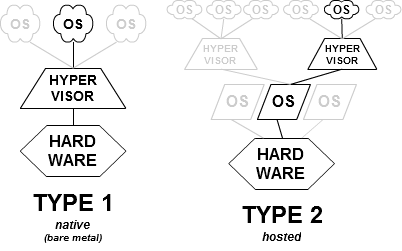
\includegraphics{Figures/hypervisor_difference.png}
\decoRule
\caption[Differences between Type 1 and Type 2 Hypervisors]{The Type 1 hypervisor, shown on the left, operates directly on computer hardware. The Type 2 hypervisor, shown on the right, is hosted on an existing operating system \parencite{Wikipedia_hypervisors}.}
\label{fig:Hypervisors}
\end{figure}

Type 1, also known as bare-metal or native. Type 1 hypervisors are run with specialised operating systems designed to give direct hardware access. This approach is generally the more efficient of the two and in some cases it can be more secure.

Type 2, or hosted, hypervisors are packaged with software that runs on a general purpose host operating system such as Microsoft Windows or general Linux distributions. Virtual machines that are run with Type-2 hypervisors are seen as processes to the host operating system. Since it shares resources with other processes that execute on the host, this is generally seen as a less efficient, but easier approach to virtualisation.

\subsubsection{Containers}

Containers are not a novel idea. Over the years there have been various isolation or containerisation techniques developed which all try to achieve secure, isolated processing environments in their own ways. These include things such as FreeBSD Jails, Linux-Vserver and Linux Containers (LXC). They are lightweight isolated spaces of resources that can be used for various things and in some cases can replace virtual machines for specific tasks. They are mainly software engines that utilise Linux kernel features in order to achieve isolation of resources and access to other processes to avoid virtualisation.

Today they are generally used to enable applications or services to be built on a variety of different system configurations without the need to worry about software dependencies. They also enable the ease of moving the application and running it on a wide variety of different systems.

\subsubsection{Differences Between Containers and Virtual Machines}

The major problem that virtual machines, henceforth referred to as VMs, have is an inherent performance hit over a single operating system, or "bare-metal" machine. Due to the implementation architecture, the hypervisor runs on or alongside the host operating system of the machine and one or more virtual machines can be created from this. Each virtual machine has its own operating system and kernel, which means that there are redundant services being executed over the machine as a whole.

Containers alleviate the resource-hungry problem that virtual machines pose by eliminating the need to run a separate instance of a guest kernel and operating system all together. Only a subset of components that make up an operating system is needed by a container, such as the libraries of the operating system image used and its own network stack, process tree, and others depending on the implementation.

The core differences between the two approaches are broken down in Figure \ref{fig:hypecont_diff}.


\begin{figure}[h!]
\centering
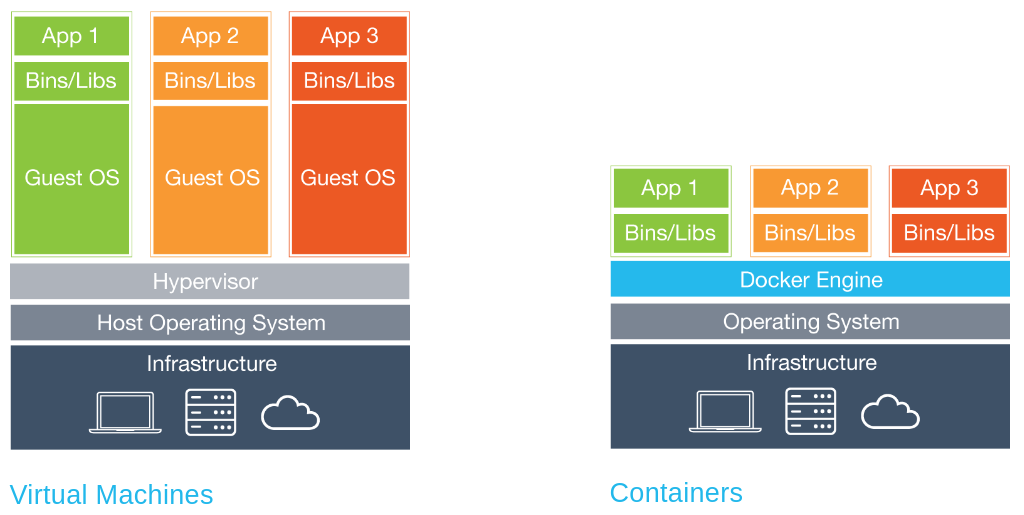
\includegraphics[width=\textwidth]{Figures/hypervisor_vs_container.png}
\decoRule
\caption[Differences between Hypervisors and Containers]{The image on the left describes the typical hypervisor-based virtual machine execution layers. The image on the right shows how container engines bypass areas of the hypervisor approach, sitting closer to the bare hardware. \parencite{enterprise_hypercont_diff}.}
\label{fig:hypecont_diff}
\end{figure}

As VMs are added to a host machine, a larger chunk of resources are reserved just for the guest operating systems themselves, leading to less resource availability for the applications or services. Not only this, but, due to the additional complexity of the VMs, they can become computationally expensive to operate in large numbers \parencite{gupta2015comparison}.

On the other hand, containers can achieve much higher density per host, that is to say that more containers can run on a single physical machine than virtual machines. Testing done for \textbf{\textit{Linux Containers and the Future Cloud}} by Rosen\footnote{Linux Containers and the Future Cloud is a presentation that was delivered for the Haifux Club at the Israel Institute of Technology on 17 March 2014. \url{http://cs.technion.ac.il/events/2014/2012/index.html}} \parencite{rosen2014linux} showed that OpenVZ and PCS achieved densities roughly 54\% and 227\% more than the best VM platform tested (RHEL KVM), respectively. 

Another advantage of containers is that the startup and shutdown time can be much faster than VMs, which can lead to higher overall time-to-business, and native nesting support (containers within containers). This is due to virtual machines needing to do the entire guest operating system boot process. However, when the working environment is of a heterogeneous nature, such as networks of systems that run operating systems other than Linux, containers can be restrictive and introduce additional complexity. Other operating system vendors have started making efforts to produce their own container systems or support existing ones, so this issue may be resolved in the future \parencite{ms_docker}.


\subsubsection{Types of Containers}

There are various container systems that are used today (\textit{vide supra}) and studies have been done to compare some of the major containers systems used in the modern world in terms of performance, features and/or security \parencite{bui2015analysis,gupta2015comparison,xavier2013performance}.

The following section mentions some of the container systems spoken about in the papers referenced above. Note that the following is not an exhaustive list of container systems nor their features.

\paragraph{Docker} \label{container:docker}
Docker is one of the most recent (2013) and popular container systems being used today. This specific one has recently enjoyed massive adoption by various types of companies and research groups, helping replace virtual machine infrastructure and creating ease of application development and deployment. It is based on LXC, another container system, but has moved from using this as its core to utilising linux control groups (cgroups) and namespaces\footnote{Control groups and namespaces are Linux kernel features that allow for isolation of resources and processes for processes.} more directly \parencite{merkel2014docker}. Docker makes use of hostname, inter-process communication (IPC), mount, network, user and process identifiers (PID) namespaces \parencite{bui2015analysis} for security and privacy as well as cgroups for resource limiting.

While it has other uses, the primary selling point of Docker is to contain a single application or portion of an application with speedy deployment. It can provide secure and robust communication between a container and its host. Each container has its own virtual network stack, unless manually specified otherwise, which takes care to abstract network traffic from the host. The organisation behind Docker provides a registry service called the Docker Hub which hosts many official and third party Docker images, which boosts the sharing capability and increases development startup time. Private registries are also available for more specialised or sensitive use \parencite{boettiger2015introduction}.

The Docker engine uses an API which allows for automation scripting and development, better management tools and reporting on containers and images. It also makes use of an abstraction layer that allows it to work on different Linux operating systems in identical fashion. To get compatibility within Microsoft Windows, Docker makes use of a hypervisor in which it gets deployed.

The main caveat with Docker is that it requires privileged user permissions on the host operating system in order for the user account to interact with the Docker system service, which takes care of launching and managing containers. This is an issue in multi-user environments.

\paragraph{Linux-Vserver} 
This is one of the oldest containerisation systems around, with the first public release in 2003 \citep{linuxvserver}. In order to use this container system, the system administrator is required to patch the host Linux kernel for their operating system in order to provide isolation between the host system and containers. This patching also enables inter-container isolation in addition to resource control \parencite{quetier2007scalability}.

It makes use of chroot calls to create a new root file system for each container\footnote{Chroot is an an isolation technique on Linux that changes the apparently root directory for a process.}. Due to the use of global PID spaces for process isolation, good performance and scalability is easy to achieve , but features such as live migration and other virtualisation features are mostly not achievable with Linux-Vserver. All containers share the same network subsystem, with identifiers added to packets to prevent snooping. This approach disallows containers from modifying their own routing tables, which may potentially limit its usefulness for tools that require unique network configurations. For CPU isolation, the Linux Scheduler is used with a Token Bucket Filter\footnote{The token bucket filter in this case is the application of the token bucket algorithm applied to the CPU scheduler.} on top of it \parencite{soltesz2007container}. Each process is linked to the creation of a token. Memory restrictions are done through rlimit, the Linux kernel system feature that controls memory usage per process or user. Recent version include cgroup support.

Linux-Vserver has proven to not be as flexible as other container systems.

\paragraph{OpenVZ}
OpenVZ is a relatively old container system, released first in 2005. It is similar to Linux-Vserver, but it uses Linux namespaces directly \parencite{dua2014virtualization}. OpenVZ treats a container as a small instance of a virtual private server (VPS) rather than as an application, as Docker does.

It uses its own custom patched Linux kernel dubbed the OpenVZ kernel which provides features such as virtualisation, isolation, resource management, and checkpointing which are common to other virtualisation platforms \parencite{kolyshkin2006virtualization,che2010synthetical}. Modern versions can use the mainline Linux kernel 3.x with a reduced feature set. OpenVZ can also be limiting to certain application due to the restrictions placed on the kernel requirements. All containers on a single host use the same kernel and architecture. Each container has its own process tree, serial ports, file system and network stack, although the host's network stack can be passed through to containers.

\paragraph{LXC}
LXC, or Linux Containers, is a newer container technology which was first released in 2008. It makes use of namespaces, in similar fashion to Docker, since Docker was based on LXC. Cgroups are utilised to provide resource management and I/O (input/output) operations are done through the Completely Fair Queuing (CFQ) scheduler \parencite{rizki2016performance}.

With some configuration LXC allows containers to be executed by unprivileged users \parencite{linuxcontainerscom}. This is especially useful in multi-user environments such as high performance computing (HPC) centers, where many users are on the same machine and have potentially sensitive information to process.

It works at a significantly lower level than container systems such as Docker, having less abstraction and in turn a steeper learning curve. This also makes it possible to achieve better performance.

\paragraph{Solaris containers/zones}
Solaris zones are around the same age as OpenVZ, being made available in 2005. It was specifically designed by Oracle to be used with Solaris OS and was offered to clients who were using the Solaris environment. 

Originally designed to improve on the administrative ease and feature set of Linux-Vserver and FreeBSD jails available at the time, it attaches zone identifiers to processes in order to limit visibility of other processes, effectively hiding a process running in one zone from another. It takes advantage of many native features of Solaris such as entitlement, limits and partitions in order to do resource management \parencite{price2004solaris}.

Its main drawback is that it can not be used with other operating system environments outside of the scope of Solaris OS. This severely limits its adoption and eliminates its use in the majority of high performance computing environments.

\paragraph{Singularity}
This is the newest major container platform, publicly appearing around October 2015. Its primary use case is aimed at computational portability. The focus for this container technology has been towards researchers and scientific application from the beginning, adopting technologies and improvements that directly improve the use of these applications within the containers. Examples of this are GPU support from within containers as well as being able to utilise technologies such as MPI natively \parencite{arango2017performance,benedicic2017portable}.

Singularity does not require special privileges to execute. This is very beneficial to multi-user environments. It also has the ability to convert Docker container images to be used in Singularity, which ensures a large range of base applications and good compatibility. Process namespace isolation is used to its fullest extent by default with Singularity and it has transparent networking. Each container shares its environment with the user that started it, which makes it simpler to use from a user perspective \parencite{xavier2013performance}. It is also integrated in various workflow software and schedulers.

% For the purpose of this work, Docker and Singularity were identified as particularly useful container systems due to their adoption and usability in scientific research. 

%----------------------------------------------------------------------------------------

\subsection{High Performance Computing}

High performance computing (HPC) is the paradigm where multiple powerful computing systems are networked together in order to run problems that are computationally expensive or that have extremely large sets of data, in more reasonable time. Software for HPC environments needs to be specifically designed with parallelism in mind, as compute is executed over various different computing hosts in the network at the same time.

These environments are provided either by a university, computing research institution, private business or the research group itself.

\subsubsection{Virtualisation in HPC}

Due to the performance overheads of virtualisation, it is not commonly implemented in serious HPC environments. Few groups have attempted to make virtualisation a viable option for HPC. A notable example of this is the group ScaleMP. Founded in 2003, their mission was to create a hypervisor that spans multiple physical machines. This allows the user to get a singular view of multi-machine clusters, by pooling resources from all of them, which could simplify writing high performance applications to only have to deal with the view of one operating system instance.

In 2014, Dell published a blog post showing their experiments with traditional virtualisation in an HPC environment by using various different scientific benchmarks. They concluded the generally accepted outcome that, given an even playing field in terms of hardware resources, virtual machines tend to perform slower than running the task on the bare machine \parencite{dell_container_perf}.

\subsubsection{Containers in HPC}

There are two main container projects that are currently considered for high performance work, namely Docker and Singularity. Docker is the largest of the two (see \nameref{container:docker} in section \ref{container:docker}), given that it is mature and has been operational for many years. The other project, Singularity, is a fairly young, but promising new container engine. Singularity is more specifically targeted at scientific workflows and has native support for HPC-specific hardware whereas Docker does not, as it is targeted more at microservices\footnote{Microservices is a software development paradigm in which a normally tightly coupled software architecture is split into multiple loosely coupled components.}. However, due to Docker being more mature it has also amassed a large number of pre-built scientific containers that can easily be downloaded from the Docker Hub registry. Singularity is especially attractive for the HPC space due to it not requiring elevated privileges to run software, reducing security concerns, and its ability to support Docker images.

Docker has made a significant impact on the Linux developer community with the ease of building, shipping and managing software dependencies in applications. However, as had also been expressed that this "revolution" \parencite{jacobsen2015contain} has yet to make a meaningful impact on the high performance computing community \parencite{yu2015building,xavier2013performance}.

Aside from the benefit of having software dependencies that are easier to manage by packaging the specialised software into container images, there are more low level advantages to using a container approach to building software for HPC clusters. Software containers can allow performance levels much closer to a bare-metal system than a virtual machine with a hypervisor can, which makes it very attractive from a compute standpoint. In the white paper\footnote{A white paper in the technology industry is a technical document that describes how a technology or product solves a particular problem. \url{http://www.investopedia.com/terms/w/whitepaper.asp}} \textbf{\textit{Containerization of High Performance Compute Workloads using Docker}} by Christian Kniep \parencite{kniep2014containerization}, it was found that it is even possible to achieve better performance in a Docker container than the bare-metal operating system it resides on in some cases, due to different libraries being used by the container operating system.

A prototype Docker-powered HPC Cluster has also been designed and implemented, spread over different physical machines, making some modification to the network bridge to get them to work together. It was deemed feasible to implement such a system and should be considered for future work management/orchestration engines and friendly graphical interfaces \parencite{yu2015building}.

Due to the ability to wrap workflows and work environments into a highly portable package, these container technologies also become attractive as they reduce the work necessary by system administrators and managers in order to ensure that user software dependencies are met.

\subsubsection{Research}

HPC environments are generally suited to a limited set of work. Massively parallel-capable tasks benefit greatly from the services that these centers provide to their users. The current model of HPC for researchers dictates that there must be at least one system administrator available on the project who installs and manages software that is approved for use with the institution. Users are able to request software that they wish to use for installation, but there is no guarantee that it will be supported by the HPC centre. Other than using official support channels in order to support researcher workflow or pipeline, there is no way to engage with the system and make changes required by the researcher. HPC centers are generally considered to be restrictive.

%----------------------------------------------------------------------------------------

\subsection{Cloud Computing}

Before common availability of the internet as we know today, companies used to buy and maintain mainframe computers that were tasked with all the business-supporting activities that could be programmatically represented. This moved into distributed computing where multiple machines would be bought and networked in order to perform tasks together. Organisations began to offer computing time on their own servers to other parties for a price, this developed into what is known today as cloud computing. 

In layman's terms, computing infrastructure is hosted by a company or organisation and provided to end-users through an abstracted interface, known as Infrastructure as a Service (IaaS). Most cloud providers will offer one or more types of services, such as Infrastructure, Platform or Software as a Service. Each of the services offer varying levels of access to the operating system environment directly, with IaaS offering the closest to actual server access. The purpose of this is to allow people to make use of hardware infrastructure without the need to provision, manage or maintain them physically.

\subsubsection{Micro-cloud}

A relatively new paradigm, "micro-cloud" or "micro-clouds" is bringing the idea of shipping code, or applications, instead of data to be processed at different locations. The paper \textbf{\textit{Mobile Micro-Cloud: Application Classification, Mapping, and Deployment}} \parencite{wang2013mobile} defines a micro-cloud as a "logical network" which consists of two main parts. The first is a "core" or central platform where the data set to be processed resides in its entirety. The second part consists of one or more "edge" platforms or small segments of computing power scattered across different locations, internally or externally, which deal with a need-to-know base of information from the core which is required for computing the task given to it.

The term "micro-cloud" was spawned from the paradigm of cloud computing, and describes the shift from using infrastructure hosted at and owned by a particular institution to using the infrastructure of another company over the internet. In this model an organisation does not pay for the installation cost and maintenance of hosting physical servers, instead they pay a monthly or sometimes yearly rate to a cloud computing provider such as Google or Amazon.

Security concerns arise with data being processed in areas that are possibly not owned by the data-holder. A good security model for the data needs to be available in the system as to prevent leaking of sensitive information. An authorisation and authentication system is also important for scenarios where specific people are allowed specific access to data. 

\subsubsection{High Performance Cloud Computing}

High Performance Cloud Computing, or HPC2, is an emerging trend. Cloud computing is becoming increasingly viable for some types of research, as the pay-as-you-use model offers some real value over the need to have a physical set of hardware at the institution. Any research that requires the processing of large or many data sets have the potential to benefit from this approach as cloud providers provide powerful virtual environments that are more catered to compute-heavy workloads. It also allows the flexibility and freedom of full control over the software stacks used. Some modern cloud computing providers are offering "Cluster Computing Instances" or high powered virtual machine instances that are connected to high speed interconnects. This model has proven viable for many types of research computing \parencite{hazelhurst2008scientific}.

Research has shown that HPC2 offerings are not yet on par with non-virtualised physical high performance environments \parencite{jackson2010performance}, so there is still work to be done in order to bridge the gap between purely virtualised cloud computing providers and high performance bare-metal machines. Projects have emerged in attempt to address some of the issues with access to high performance devices for virtualised environments, one such being a novel approach to using high speed compute cluster network interconnects in a cloud environment \parencite{mauch2013high}.

\subsubsection{Issues With Cloud Computing in Research}

There are various reasons why an organisation would not be able to use a conventional cloud computing platform to provide their products and/or services. Running costs, internet access, scale or privacy issues of using the cloud are among some of the reasons an organisation's internal ability to manage those aspects may outweigh the attraction of use.

Smaller organisations benefit greatly from utilising the offerings of cloud environments due to the high cost of infrastructure acquisition, but subscription costs for storage and compute will continue to grow as time progresses. The potential to become more costly to maintain a cloud environment than a physical one increases when organisations want to scale their services or utilisation. Some flexibility is also sacrificed as users have no physical access to any of the hardware that they are renting, which results in users having to work around restrictions or limitations that are in place with cloud environments. This issue is constantly being worked on by cloud environment providers by offering increasing amounts of customised solutions for various use cases as evident by regular releases of new platforms and tools by said providers\footnote{The work being done by the three most successful cloud computing provides can be found at the respective blogs: Google (\url{https://cloudplatform.googleblog.com}), Amazon (\url{https://aws.amazon.com/blogs/aws/}) and Microsoft (\url{https://azure.microsoft.com/en-us/blog/}).}.

Privacy is another fairly serious concern with cloud environments. When data is stored on cloud environments, the user is subject to the privacy policy and terms of use of the cloud provider. The user is also subject to housing the data they wish to store on one or more of the physical locations that a cloud provider may offer. Data centers are not available in every country or continent. This has potential ramifications for data that is governed with strict policies, where there is no strict control of how data is stored and/or replicated by the cloud provider \parencite{abouelmehdi2017big}. Lawmakers are catching up to the notion of privacy-centric data and location agnostic cloud environments \parencite{gholami2016big}. Researchers themselves can take preventative steps to protecting their data as well with approaches such as data segmentation, encryption and anonymity masking \parencite{sun2014data}. Unfortunately there is no concrete solution to data placement laws, short of having cloud providers open data centers in every country in the world.


%----------------------------------------------------------------------------------------

\subsection{Workflow Languages}

Bioinformatics data often needs to go through various steps of transformation to be usable for different purposes. While some pipelines or workflows are presented and shared as a structured set of tools that need to be executed in a specific order, many researchers chain tools together in novel ways to achieve their own goals. A large percentage of students and researchers in this space are not programmers \parencite{mesirov2010accessible}. Many researchers and students in the field of bioinformatics perform data analysis by using programming languages including, but not limited to Python, R, or Bash to write scripts that are highly specific to the tools, data and environment that they are working on. There is a growing problem with these pipelines not being easily reproducible or extensible by others. Implications of this are that it becomes difficult to verify whether the results of other researchers are correct and to expand on the groundwork that others may have laid with their original work.

Workflow languages offer a way to address this issue. They provide a structured way for researchers to provide the inputs, tools and outputs that are required for each possible step of an analysis. The execution tools for the specific languages allow these workflow definitions to be executed on different machines without needing to modify them for your specific environment and consequently make it significantly easier to acquire the specific tools and versions of those tools for the said workflow. Many of these workflow languages also integrate with container technologies such as Docker and Singularity to retrieve the desired tools at the time of execution.

\section{Project Aims}

There are three main research questions that this project aimed to address. The overall aim was to address these issues by providing an automated tool and simple interface for researchers to utilise the cloud for their specific needs, without the need for complicated dependency management, manual administration or technical knowledge.

\subsection{Is it feasible to move workflows/pipelines to the cloud?}
This questions tries to understand if the paradigm of moving researcher workflows to remote locations is feasible or not. This is the main focus of this project and the subsequent questions rely on this main question.

\subsection{Can the cloud environment be simplified for researchers?}
It is unreasonable to expect that most researchers understand how to use specific technologies such as cloud computing environments and specific operating systems, along with their intricacies, in order to reproduce their working environment remotely. Therefore, the remote execution environment should be simplified for use by non-technical researchers by attempting to create a structured and reproducible way for them to define their specific environment which can automatically be made for them.

\subsection{How can workflow languages be supported in the cloud?}
Standards need to be put in place in order to create redistributable workflow specifications. It is difficult to maintain a system that supports endless different workflow specifications. A balance needs to be struck with how many to support. This question asks how workflow specifications can be integrated into a cloud environment to allow for reproducible science and researcher flexibility.

The source code for the prototype software developed for this project can be found at \url{https://github.com/Banshee1221/Nikeza}.